% This is a section template for reflective journal

% Remove or comment out this whole environment when using this template.
{\begin{center}
    \textcolor{red}{\Huge{THIS IS A FILLED SAMPLE SECTION}\\[4mm] ...with realistic notes...}

    \begin{tabular}{r @{: } p{80mm}}
        {\textcolor{blue}{Blue text}} &  Help text. Short description of how to use an environment or a section in the template.\\
        <<{\emph{text placeholder}}>> & Text between angle brackets are placeholders. Indicates a string to be replaced with input text.\\
        Normal text/black fonts & Real note/example text, how the section is intended to be used.
    \end{tabular}

\end{center}

% ----> Header informaton section - Start
\section{Lesson 1: Course Introduction}

\begin{notes}[Typesetting Generic Document Elements]
    The couple of pages shows uses different \LaTeX commands to typeset a document with the most common text types.

    The document uses; Section, Subsection, quotes, italic, bold etc.
\end{notes}

Original URL: \url{https://www.noroff.no}
% <---- Header informaton - End


% ----> Main reflective subsection - Start
% ----| Write reflective thoughts on the topic in general. |----
\subsection{Reflection on the days lecture and tutorial}

Lesson 1 was an introduction on the subject of {\emph{Programming Databases}}. It gave a nice overview about the subject, how it is layed out, and perhaps most importantly the study goal. Compared to the 3 other subjects taken since the start of this course, it is the first subject where the subject was clearly outlined along with the goals.

There was a statement, see quote on page \pageref{quote} from Prof. Johan Van Niekerk, which is important to keep in the back of mind. It should perhaps be pinned to the wall as a reminder of a pitfall to be cognizant of when surmounting challenging study phases. A reminder to wisely allocate the effort exerted, and lower the level of pondering on the vastness of relevant topics, but stay in focus inside the subject domain, at hand.

The statement resonated with me personally, since I regard lack of focus and wasted effort as one culprit of my struggle to keep up on course materials and assessments. I find it very easy to veer of on a tangent and wander away from the study material. For example, making search queries and delving into statistics, while addressing probability in discrete math.

% <---- Main reflective subsection - End



% ----> Main reflective subsection - Start
% ----| Write reflective thoughts on a specific reflective topic. |----
\subsection{Reflection Topics}

None applicable for this lesson. No reflection topics given for this lesson.

% <---- Main reflective subsection - End



% ----> Key Take-Away subsection - Start
% ----| Write Itemized notes regarding the lesson topic. |----
\subsection{Key Take-Away}

\begin{table}[H]
    \begin{tabular}{p {20mm} @{: } p{80mm}}
        Lesson date & 2077 01 15 \\
        Date taken & 2077 01 15 \\
        Revisited & N/A \\
    \end{tabular}
\end{table}

Items/bullet points outlines  below outlines key information from the day's lesson.

\begin{itemize}
    \item Working with database (SQLite)
        \begin{itemize}
            \item Acquire fundamental skill about working with databases
            \item How to design as simple normalized database
            \item Understand database storage and data structure
            \item Understand database Normalization
            \item Be able to query and interface with databases
            \item How to script and automate database connection, mangagement and datamining
            \item Automate data manipulation and analysis, generating reports and statitics etc on data in databases, dataframes etc.
            \item Understanding and being able to manage and  work with databases is therefore key to the field of CyberSecurity.
        \end{itemize}
\end{itemize}

Course: UC1PR2101 - Programming Databases

\begin{enumerate}
    \item New lesson structure.
        \begin{enumerate}
            \item The course is layed out to be taken with a more individual approach, akin to remote studies. More preparation are expected prior to lecture sessions.
            \item Lessons are broken up into smaller topics.
            \item Reflective Journals are not mandated. 20\% of the mark will not be allocated to Reflective Journal submition.
            \item Quizes will be smaller and with a formative purpose. There will be a practice Quizes.
            \item Overall reduced number of submition for assessment. Course grades will be based on 1 or 2 larger assessments, instead of many smaller assessments.
            \item Course assessment targets, along with target dates to be posted soon.
        \end{enumerate}
    \item New Lecture structure.
        \begin{enumerate}
            \item Students are expected to engage with study material at least 1 day ahead.
            \item Students are expected to be more prepared for each lecture topics.
            \item Referenced resources are not "mandatory", students must choose what materials are applicable and important.
        \end{enumerate}
    \item Tools and applications
        \begin{enumerate}
            \item SQLite
            \item Python
            \item PANDAS(?)
        \end{enumerate}
\end{enumerate}

Learning Databases itself is a comprehensive part of software engineering and software development, which cannot be condensed in a 6 week course.

\begin{displayquote}\label{quote}
    {\emph{We are not software developers. Our purpose is to learn enough to be able to understand enough to know what we are looking at when we are working with someone elses (database) design templates...\\}}
    {\ttfamily{
        - Prof. Johan Van Niekerk}}
\end{displayquote}

Analogous to learning enough foriegn language; One is not expected to be a fluent speaker. But know enough, to converse and to be able to accomplish a specific goal. Deeper knowledge are obtained along the way, where fluency comes through effort and immersion over time. 

My personal take on this (to make it relatable to the course) is as follows: A car crash forrensic investigator should know enough about a car to tell the pieces from eachother, but is not expected to fix, design or engineer a car to prodution.

% <---- Key Take-Away subsection - End


% ----> Lessons Learned subsection - Start
% ----| Write a summary about the day's lesson topic. |----
\subsection{Lessons Learned}\label{sec:lessons_learned}

\begin{notes}[Typesetting Bullet-points]
    Examples below use combination of \textbackslash begin statement with \textbackslash itemize environment containing \textbackslash item command to make a bullet-point.
    
    The \textbackslash itemize environment can be nested to create a sub-bullet-point. Creating 2 levels of bullet-points.
\end{notes}

This subsection summarizes the day's lesson topic.

\begin{itemize}
    \item Why databases (in relation to CyberSecurity)?
        \begin{itemize}
            \item Acquire fundamental skills about the purpose of databases
            \item Understand how databases are key to modern data and information infrasctructure
            \item Get an overview of the majority of todays transactional databases today and their use of relational database
            \item Understand how systems and data breach are on the database connectivity and transactional level
        \end{itemize}
    \item What is a database?
        \begin{itemize}
            \item Acquire fundamental skills about what a database is
            \item What databases are used for
            \item What types of databases are in use
        \end{itemize}
    \item Where does database fit into the ecosystem of "data"?
        \begin{itemize}
            \item Be able to identify different ways of storing, structuring and organizing data.
        \end{itemize}
\end{itemize}


{\bfseries{Databases}}

Databases organize data/information by following examples.

\begin{itemize}
    \item Catagorization
    \item Quantify
    \item Itemization
    \item Relation etc.
\end{itemize}

Database systems aims to resolve some data storage issues such as problemetic {\emph{Data redundancy/duplication}}:
\begin{itemize}
    \item Storage, takes space
    \item Overhead, when updating
    \item Itegrity, data consistency
\end{itemize}

\subsubsection{NIS' objectives}

\begin{notes}[Citations]
    Examples using the \textbackslash cite command.

    The cite command can automatically populate the Bibliography on page \pageref{sec:bibliography}
\end{notes}

NIS (\cite{VIIRA2018}) Directive its annexies and Corrigendum (\cite{EuropeanCommission2017}) , a communication by the European Commission to its Member States, the Directive has 3 main objectives:

\begin{notes}[Typesetting Acronyms]
    Examples using the:
    \begin{itemize}
        \item \textbackslash arcshort
            \begin{itemize}
                \item The acronym with arcshort: \acrshort{cert}
            \end{itemize}
        \item \textbackslash acrslong
            \begin{itemize}
                \item The acronym with arclong: \acrlong{cert}
            \end{itemize}
        \item \textbackslash acrfull
            \begin{itemize}
                \item The acronym with arcfull: \acrfull{cert}
            \end{itemize}
    \end{itemize}
\end{notes}

\begin{itemize}
    \item Improving nationanl cyber security capabilities,
    \item Building cooperation at EU level, and
    \item Promoting a culture of risk management and incident reporting among key economic actors, notably \acrfull{oes} for the maintenance of economic and scietal activities and \acrfull{dsp}.
\end{itemize}

However, each Member State are expected to expand on the 3 main objectives, and define its \acrshort{ncss} according to each Member State's specific needs and priorities as long as it is never below the requirements and objectives set in the NIS Directive.

\begin{notes}[Typesetting Glossary]
    Examples using the \textbackslash gls command.

    Using the glossary enables you to use a term inline, and create a Glossary index using the \textbackslash printglossary[title=Glossary, toctitle=Glossary] on page \pageref{sec:glossary}

    Using the glossary also enables you to use a term inline, and create an Acronym index using the \textbackslash printglossary[type=\acronymtype] on page \pageref{sec:acronym}

    \textcolor{red}{Beadvised:} Please make sure to read the official "glossaries" CTAN package. There are some quirks that is nice to be aware of. The most important is the following.

    Rendering a PDF referring to a glossary or acronym that does not exist will result and error.

    To generate the acronym and glossary index correctly, \textcolor{red}{execute sequence below accordingly. Take note that the file name \emph{document} omits the .tex part of the file name.} 
    
    \begin{itemize}
        \item Run the \textcolor{green}{\ttfamily{pdflatex document}} (or simply save the file if you are using VS-Code) to trigger the Glossaries package. The pdflatex will parse all of the \textbackslash gls and \textbackslash acr commands. A reference will be created to be used with the makeglossarie command.
        \item Run the \textcolor{green}{\ttfamily{makeglossaries document}} to generate an index using the glossary.tex of defined glossaries and acronyms. 
        \item Re-run the \textcolor{green}{\ttfamily{pdflatex document}} (just save again with VS-Code)to render the DPF with the glossary.tex is used with correct references in the PDF file.
    \end{itemize}
\end{notes}


We will now use the term \Gls{directive} inline, using the \textbackslash Gls command. Which will use the glossary.tex file and automatically populate the Glossary section on page \pageref{sec:glossary}.

Here we use another term; \gls{transposition}, example using Glossary module. It will be the second item to be listed in the Glossary index


{\bfseries{Glossary:}}

\begin{notes}[Typesetting Table 1]
    Below is an example of a manually built "Glossary" using the \textbackslash begin statement with the \textbackslash tabular environment to create a table.

    The disadvantage of manually creating a glossary table is that is will not be indexed. 
\end{notes}

\begin{tabular}{p{40mm} | p{120mm}}[H]
    {\bfseries{Key Word/Expression}} & {\bfseries{Elaboration/Comment}}\\ \hline
    Database & A logical way to organize, store, label and describe relationships of data.\\ \hline
    Third Normal Form & Relational databases. A database schema design see "Other source material" table in section \ref{subsec:source}. Ensures update and insert integrity to the database.\\ \hline
    (Working in) Disconnected mode & A safe way to work with data in Databases, to avoid data curruption or data integrity error. Such curruption or error can occur when multiple connections are made and edits the same data at the same time. Tracking which changes, by which connections, is the most recent and valid change will be difficult. Working in "Disconnected Mode" will remedy this issue.\\ \hline
    SQL & {\bfseries{S}}tructured {\bfseries{Q}}uery {\bfseries{L}}anguage - a standardized language to interface with databases\\ \hline
    DDL & {\bfseries{D}}ata {\bfseries{D}}efinition {\bfseries{L}}anguage - tells a database how it data will be stored or organized. \\ \hline
    DML & {\bfseries{D}}ata {\bfseries{M}}anipulation {\bfseries{L}}anguage - tells the database how to operate the data. \\ \hline
    Database Normalization & Structuring a relational database, reduce data duplication and improve data integrity. \\ \hline
\end{tabular}

\begin{notes}[Typesetting graphics][H]
    Below are a couple of examples useing the combination of \textbackslash begin statement, \textbackslash figure to create an environment where the \textbackslash includegraphics command is used to insert graphics in a \LaTeX document.
\end{notes}

{\bfseries{Graphics with .png files}}

\begin{figure}[H]
    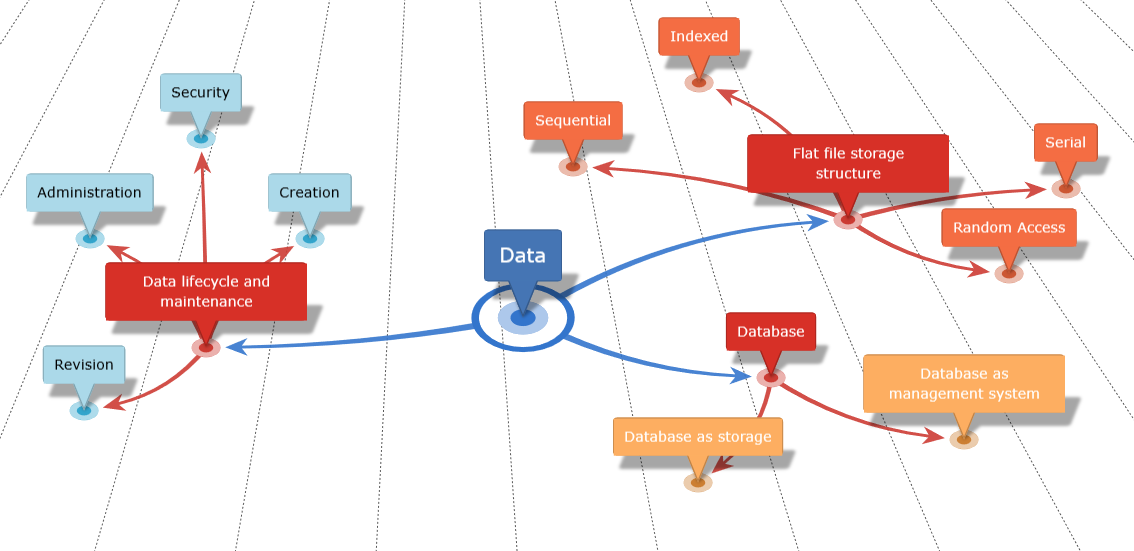
\includegraphics[width=\linewidth]{tex/Data_cropped.png}
    \caption{Data Mindmap}
    \label{fig: Data Mindmap}
\end{figure}

\begin{figure}[H]
    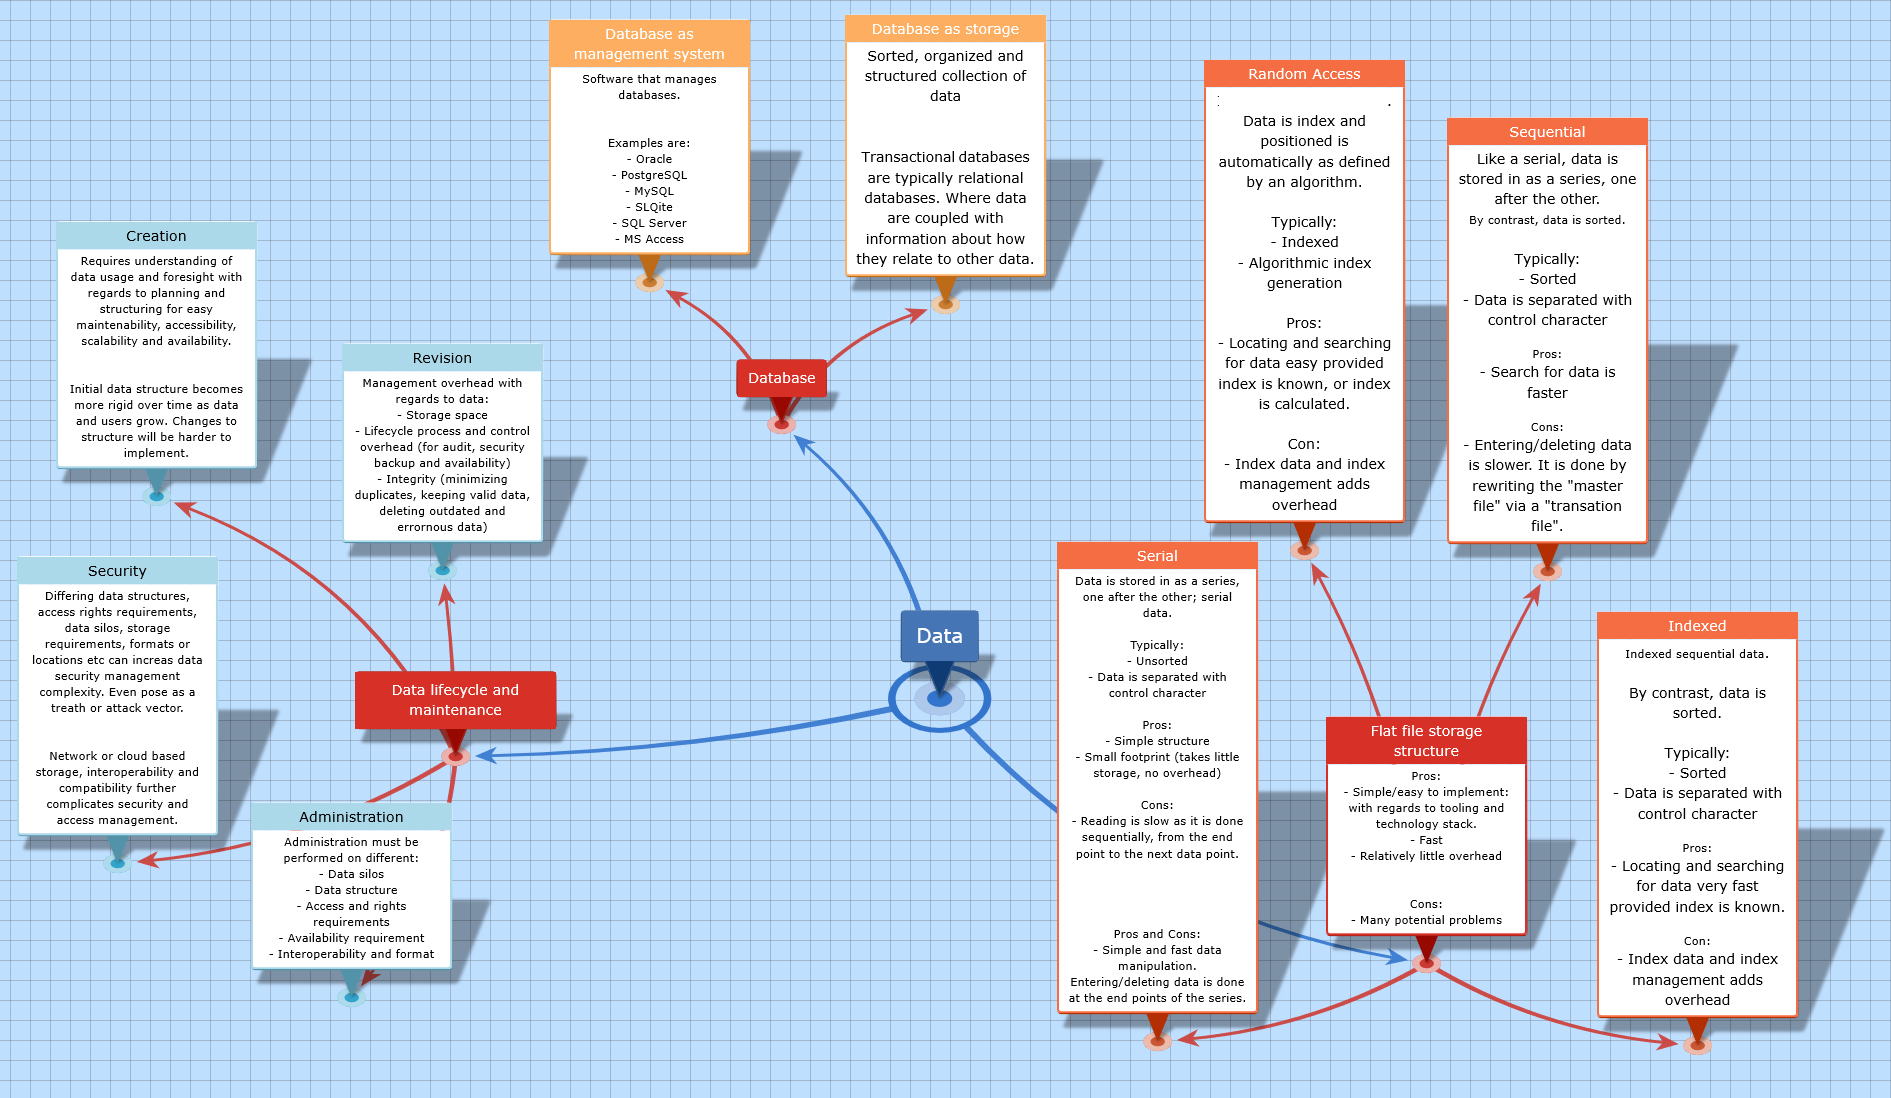
\includegraphics[width=\linewidth]{tex/Data_cropped2.png}
    \caption{Data Mindmap - with detailed notes expanded}
    \label{fig:Data Mindmap expanded}
\end{figure}

% <---- Lessons Learned subsection - End


% ----> Action-Point subsection - Start
% ----| To-do list to complete the day's lesson topic. |----
\subsection{Action Points - Further Reading/Enquiry}

\begin{notes}[Typesetting Table 2]
    Below are two tables, a "to-do" and a resource list, using the \textbackslash begin statement with the \textbackslash tabular environment to create a table.

    Tables in the examples below are using manually set column formatting. In addition to the "adjustbox" environment.
\end{notes}

\begin{adjustbox}{max width=\textwidth}
    \begin{tabular}{c|l|l|c|l}
        {\bfseries{Action Point}} & {\bfseries{To-do description}} & {\bfseries{Assigned to}} & {\bfseries{Target date}} & {\bfseries{Comment/Status}} \\
        \hline
        1 & Verify/enroll to Teams channel membership for the course & N/A & ASAP & Assigned \\ \hline
        2 & Setup a home-lab with SQLite & N/A & ASAP & Assigned \\ \hline
        3 & Look up and learn SQL (DDL, DML etc) & N/A & ASAP & Assigned \\ \hline
        4 & Look up and learn UML & N/A & ASAP & Assigned \\ \hline
    \end{tabular}
\end{adjustbox}

% <---- Action-Point subsection - End



% ----> Other source materials subsection - Start
% ----| A list of materials not directly provided via the course books/distributed by lecturers for the day's lesson topic. |----
\subsection{Other source materials} \label{subsec:source}

\begin{tabular}{p{40mm} | p{120mm}}
    {\bfseries{Resource Type}} & {\bfseries{Source description, Book title, URL, etc.}}\\
    \hline
    Wikipedia - 3rd Normal Form & \url{https://en.wikipedia.org/wiki/Third_normal_form}\\ \hline
    Wikipedia - SQLite & \url{https://en.wikipedia.org/wiki/SQLite}\\ \hline
    Youtube - SQLite & \url{https://www.youtube.com/watch?v=byHcYRpMgI4}\\ \hline
    YouTube - SQLite usecases & \url{https://www.youtube.com/watch?v=Jib2AmRb_rk}\\ \hline
    SQLite - Official & \url{https://sqlite.org/index.html}\\ \hline
\end{tabular}

% <---- Other source materials subsection - end


% ----> Issues Noted and Area of Improvements subsection - Start
% ----| A list of items, after-thought about issues, difficulties (on the subject itself, materials, tools, etc.) working with the day's lesson topic. |----
\subsection{Issues Noted and Area of Improvements}

\begin{tabular}{c|l}
    {\bfseries{Issue number}} & {\bfseries{Issue description / Area of Improvement}}\\
    \hline
    1 & N/A\\ \hline
    2 & N/A\\ \hline
    
\end{tabular}


% <---- Issues Noted and Area of Improvements subsection - End